\section{Arquitectura del sistema}

\noindent
La arquitectura de software es el diseño de más alto nivel de la estructura de un sistema. Una arquitectura de software consiste en un conjunto de patrones y abstracciones coherentes que proporcionan un marco definido y claro para interactuar con el código fuente del software.
\newline 
A continuación, se muestra la arquitectura que define a ESCOMobile, en donde se pueden observar los componentes y su interacción.

\pagebreak
\begin{figure}[!htpb]
	\hypertarget{fig:Arqui}{\hspace{1pt}}
	\begin{center}
		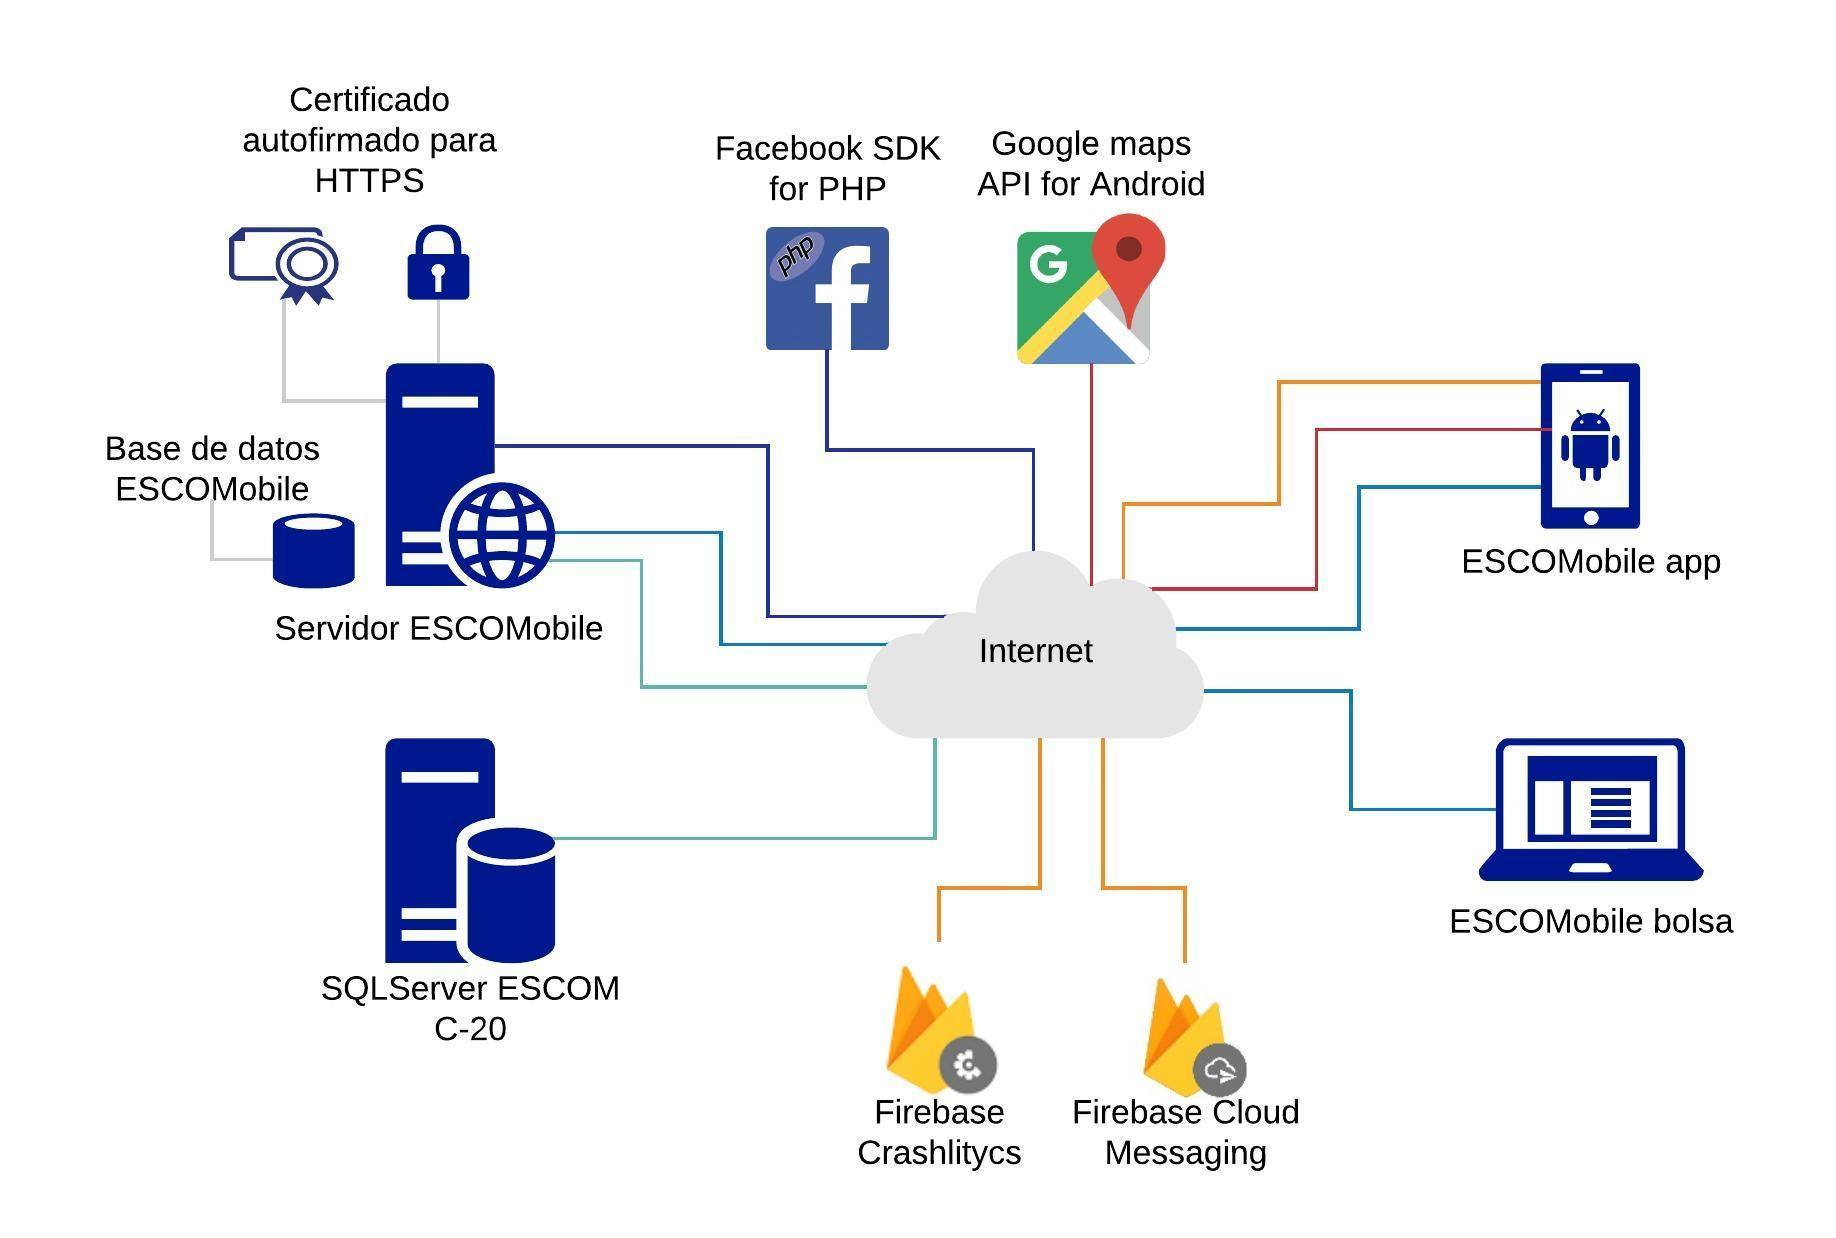
\includegraphics[width=1\textwidth]{images/clases/arquitectura}
		\caption{Arquitectura de ESCOMobile.}
		\label{fig:Arqui}
	\end{center}
\end{figure}